\chapter{Quick Start Example}
% Again a short introduction.
This chapter starts with some instructions on how to download and install Kieker %
in Section~\ref{sec:example:downloadInstall}. %
Using a simple Java example, the following Sections~\ref{sec:example:monitoring} %
and \ref{sec:example:analysis} demonstrate how to use \Kieker{} for monitoring %
and analyis. %
% Notify-tag because this could be interesting for the reader.
\notify The presented Java sources are included in the \Kieker{} release.

\section{Download and Installation}\label{sec:example:downloadInstall}

The \Kieker{} release distribution can be downloaded from \KiekerURL. The web %
site provides zip/tar.gz archives of the \Kieker{} binary distribution as well %
as the corresponding \Kieker{} source code archives.

For this chapter, it is required to download and extract an archive containing %
Kieker's binary distribution, e.g., \file{kieker-\version{}\_binaries.zip}.
The extracted content should have the following directory structure:

\vspace{1ex}
\dirtree{%  
.1 kieker-\version{}/.
.2 bin/\DTcomment{Some wrapper scripts for \Kieker{} tools}. 
.2 dist/\DTcomment{The \Kieker{} libraries required for monitoring and analysis}.
.3 \analysisJar\DTcomment{}.
.3 \commonJar\DTcomment{}.
.3 \monitoringJar\DTcomment{}.
.3 \toolsJar\DTcomment{}.
.2 lib/\DTcomment{Libraries required by Kieker}.
.2 META-INF/\DTcomment{Example configuration files}.
} 
% Linebreak because the text would be to close to the directory tree. 		


% If desired, the new created directory can be assigned to an easy remindable environment variable.
	\section{Monitoring}\label{sec:example:monitoring}
		For the creation of the example is is recommended to create a new working directory (e.g. \dir{example}) of the following structure:
		\dirtree{%  
		.1 example/\DTcomment{The root directory of the project}.
		.2 build/\DTcomment{The directory for the compiled class files for Java}. 
		.2 lib/\DTcomment{The directory for the libraries and needed jar-files}.
		.3 \monitoringJar\DTcomment{}.
		.3 \commonJar\DTcomment{}.
		.3 commons-logging-1.1.1.jar\DTcomment{}.
		.2 src/\DTcomment{The directory for the sourcecode files}.
		.3 mySimpleKiekerExampleManual/\DTcomment{The directory for the new package}.
		.4 CRM.java\DTcomment{One of the sourcecode files}.  
		.4 Catalog.java\DTcomment{One of the sourcecode files}.
		.4 Bookstore.java\DTcomment{One of the sourcecode files}.
		.4 BookstoreStarter.java\DTcomment{One of the sourcecode files}.
		} 
		% Linebreak because the text would be to close to the directory tree. 		

		The listed jar-files must be copied from the \Kieker\  directory:
		\begin{itemize}
			\item \dir{\KiekerDir/dist/\commonJar}
			\item \dir{\KiekerDir/dist/\monitoringJar}
			\item \dir{\KiekerDir/dist/commons-logging-1.1.1.jar}
		\end{itemize}
		The following listings show the content of the sourcecode files:
		\setJavaCodeListing       
		\lstinputlisting[caption=Bookstore.java]{source-example/manual-monitoring/src/mySimpleKiekerExampleManual/Bookstore.java}
		\begin{lstlisting}[caption=BookstoreMonitoringStarter.java] 
package bookstoreApplication;

import kieker.monitoring.core.MonitoringController;

public class BookstoreStarter {

    public static void main(String[] args) {
        Bookstore bookstore = new Bookstore();
        for (int i = 0; i < 5; i++) {
            System.out.println("Bookstore.main: Starting request " + i);
            bookstore.searchBook();
        }
}
\end{lstlisting}
		\lstinputlisting[caption=CRM.java]{source-example/manual-monitoring/src/mySimpleKiekerExampleManual/CRM.java}

		\lstinputlisting[caption=Catalog.java]{source-example/manual-monitoring/src/mySimpleKiekerExampleManual/Catalog.java}

		The monitoring itself is done manually. Although this is not the strength of \Kieker\ it is pretty good for a quick start. 

		% Make sure that this listing will be modified, once the sourcecode changes!!!
		% It must show the whole monitoring of the bookstorecall, from getting the first time to persisting of the record!!
		\lstinputlisting[firstline=20, lastline=29, caption=Cutting from Bookstore.java, label=listing:cuttingBookstore]{source-example/manual-monitoring/src/mySimpleKiekerExampleManual/Bookstore.java}
		
		In Listing \ref{listing:cuttingBookstore}  can be seen, how the monitoring itself is done. The time before and after a specific method call (in this case: \method{searchBook()}) is remembered. These informations are stored in the so called operation execution record. Its (partially) layout can be seen in Figure \ref{Figure:OperationExecutionRecordClassDiagram}.

		\begin{figure}[H]
			\begin{centering}
				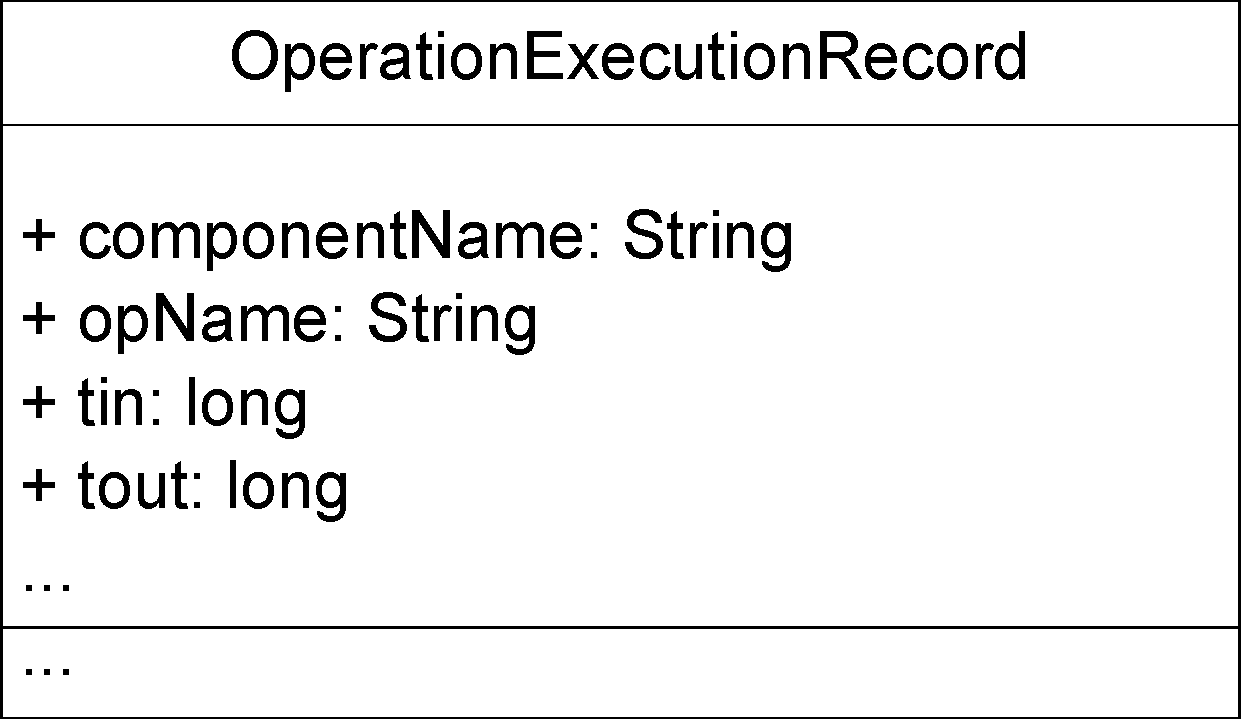
\includegraphics[width=0.4\textwidth]{images/OpExRecClassDiagram}
				\caption{The class diagram of the operation execution record}
				\label{Figure:OperationExecutionRecordClassDiagram}
			\end{centering}
		\end{figure}

		The important attributes for now are:
		\begin{itemize}
			\item componentName: The component (the class) in which the called method is.
			\item opName: The called method.
			\item traceId: The trace id of the current trace we want to record. Due to the fact, that we follow only one trace, this is zero in all recordings.
			\item tin: The time before the sourcecode which should be measured.
			\item tout: The time after the sourcecode which should be measured.
		\end{itemize}
		The sourcecode should now be compileable and executable:

		\setBashListing 		
		% Note: This is different under Windows and Linux!! 		
		% If the Kieker-Dir for the tutorial is changed, make sure that this is done here as well!! 		
		% We cannot put a latex-macro within the listing!
		\begin{lstlisting}
nils@Laptop:~/example$ javac src/mySimpleKiekerExampleManual/*.java\
 -classpath ./lib/°\commonJar°:./lib/°\monitoringJar°:\
 -d build

nils@Laptop:~/example$ java\
-classpath ./build/:\
./lib/°\commonJar°:./lib/°\monitoringJar°:./lib/°\commonsLoggingJar°\
mySimpleKiekerExampleManual.BookstoreMonitoringStarter 
\end{lstlisting}
			

		% warning-tag because windows has to be handled different.
		\warning If the sourcecode should be compiled and executed under Windows, the paths have do be sepereated with semicolons instead of colons. Furthermore it is not possible to wrap the single parts of the commands with a backslash.\\
		If everything worked correctly, there should now be a new directory with the name \dir{tpmon-20100605-115948636-UTC} (just with other numbers) in the default temporary directory (under Linux this should be \dir{/tmp}; under Windows \dir{C:/temp}). In this directory, there should be a file with the extension \dir{.dat} which contains the recorded informations from the source code. A possible content of this file can be found in the appendix of this tutorial.\\
		We take now a closer look at the analysis.

	\section{Analysis}\label{sec:example:analysis}
		As mentioned in the beginning of this chapter, it is shown how a simple consumer is programmed before starting the analysis. Therefore we need some new files:

		\dirtree{%  
		.1 example.
		.2 build. 
		.2 lib.
		.3 \monitoringJar.
		.3 \color{red}\analysisJar.
		.3 \commonJar.
		.3 commons-logging-1.1.1.jar.
		.2 src.
		.3 mySimpleKiekerExampleManual.
		.4 CRM.java.  
		.4 Catalog.java.
		.4 Bookstore.java.
		.4 BookstoreStarter.java.
		.4 \color{red}Consumer.java.
		}      
		
		The new jar-file can again be found in \dir{\KiekerDir/dist}. Listing \ref{listing:Consumer} shows the content of the new created \dir{Consumer.java}. It implements the \class{IMonitoringRecordConsumerPlugin} and overrides the necessary methods so that it can later be used by the analysis component of \Kieker. In this case the component gets a maximal response time within the constructor which will later be used to check whether a recorded method call replied fast enough or not. If the method call needed more time to response that the maximal allowed response time, it will be written directly to the error stream.\\
		The methods \method{terminate} and \method{execute} don't do anything due to the fact that the consumer doesn't need any initialization. If the consumer would for example use threads then these methods would be the correct location to start and stop them.

		\setJavaCodeListing       
		\lstinputlisting[caption=Consumer.java, label=listing:Consumer]{source-example/manual-monitoring/src/mySimpleKiekerExampleManual/Consumer.java}

		We have now to extend the file \dir{BookstoreStarter.java} to analyze our recorded informations.

		\setJavaCodeListing       
		\lstinputlisting[caption=BookstoreStarter.java]{source-example/manual-monitoring/src/mySimpleKiekerExampleManual/BookstoreStarter.java}

		% notify-tag because this is a description how the analysis works.
		\notify The analysis consists of the following steps:
		\begin{itemize}
			\item Create a new instance (or more) of the class \class{AnalysisInstance}.
			\item Register the plugins which should evaluate the records.
			\item Register exactly one reader to read the stored informations.
			\item Start the analysis instance.
		\end{itemize}
		The sourccode can now be executed:

		\setBashListing 		
		% Note: This is different under Windows and Linux!! 		
		% If the Kieker-Dir for the tutorial is changed, make sure that this is done here as well!! 		
		% We cannot put a latex-macro within the listing!
		\begin{lstlisting}[caption=Commands to compile and run the analysis under \UnixLikeSystems{},label=lst:bookstoreAnalysisStarterLinux] 			
#\lstshellprompt{}# mkdir build
#\lstshellprompt{}# javac src/kieker/examples/userguide/ch2bookstore/manual/*.java 
        -classpath lib/#\mainJarEMF# -d build/

#\lstshellprompt{}# java -classpath build/:lib/#\mainJarEMF#
       kieker.examples.userguide.ch2bookstore.manual.BookstoreAnalysisStarter 
       /tmp/kieker-20120402-163314855-UTC-myHost-KIEKER-SINGLETON
\end{lstlisting}			

		If everything worked correctly, the consumer should write something on the outputstream for every record it gets. A possible display of the run can be found in the appendix of this tutorial. 